\section{Loi conditionnelle}

Conditioning is the operation of revising a loi once part of the outcome is
known. In the discrete chapter it was an elementary quotient: the probabilité
conditionnelle of $B$ given $A$ was $\prob(A \intersect B)/\prob(A)$, and nothing
more was needed because the événements one conditions on are atoms with positive
probability. The moment variables aléatoires have densités that quotient breaks
down. The événement $\{Y = y\}$ is négligeable for every $y$, its probability is
zero, and the quotient is $0/0$; yet everyone wants to speak of the loi of $X$
given $Y = y$, and every exam problem in this course asks for one.\\

This chapter builds the object that survives the degeneracy. The route is the
one the intégrale de Lebesgue makes available: instead of dividing by
$\prob(Y = y)$, one observes that the map $B \mapsto \prob_{X,Y}(A \times B)$ is
dominated by $\prob_{Y}$, so by the théorème de Radon-Nikodym it has a densité with
respect to $\prob_{Y}$, and that densité --- read as a function of $y$ --- is
declared to be the loi conditionnelle. The price of the construction is a
qualification that never goes away: the loi conditionnelle exists and is determined
only for $\prob_{Y}$-almost every $y$. That qualification is not decoration, and it
is the reason the statements below are all phrased with an ``almost every''.\\

The plan is three steps of increasing generality: conditioning on a single
événement non négligeable, which is chapter 1 re-read with an integral in place of a
sum; conditioning on a variable aléatoire, where the loi conditionnelle appears as a
densité with respect to $\prob_{Y}$; and the case where the loi jointe has a
densité, which is the computational case the exercises live in. Espérance
conditionnelle follows, defined as an integral against the loi conditionnelle, and the
chapter closes on the tower property $\expec(X) = \expec(\expec(X \mid Y))$ with
its proof, the standard four-rung ladder of the course.

\begin{remark}
  This course builds espérance conditionnelle \emph{from} lois
  conditionnelles: $\expec(\phi(X,Y) \mid Y = y)$ is by definition an integral
  of $\phi(\cdot,y)$ against the mesure $\prob_{X \mid Y = y}$. Other
  treatments define espérance conditionnelle abstractly rather than from
  lois conditionnelles; that route is not taken here, and nothing below depends
  on it.
\end{remark}

\subsection{Condition sur un événement non négligeable}

On commence par le cas simple où la condition porte sur un événement de
probabilité non nulle. Soit $(\Omega,\mathcal{F},\prob)$ un espace de probabilité et
$A \in \mathcal{F}$ un événement tel que :
\[
  \prob(A) > 0 .
\]
La probabilité conditionnelle $\prob(\cdot \mid A)$ définit une nouvelle mesure de
probabilité sur $(\Omega,\mathcal{F})$, the same espace mesurable :
\[
  \forall B \in \mathcal{F}, \qquad
  \prob(B \mid A) \;=\; \frac{\prob(A \intersect B)}{\prob(A)}
  \;=\; \int_{B} \frac{\indic_{A}}{\prob(A)} \, d\prob .
\]
The second form is the one that generalises. It says, of
$\prob(\cdot \mid A)$ : c'est une mesure de densité
\begin{equation*}
  \omega \longmapsto \frac{\indic_{A}(\omega)}{\prob(A)} ,
\end{equation*}
par rapport à $\prob$, and everything in this subsection is a consequence of that
single sentence read through the results of chapter 3 on mesures à densité.\\

Soit $X$ une variable aléatoire à valeurs dans un espace mesurable
$(E,\mathcal{E})$ --- not necessarily real, at this stage.

\begin{definition}[Loi conditionnelle sachant un événement]
  On appelle loi conditionnelle de $X$ sachant $A$ la mesure de probabilité
  $\prob_{X \mid A}$ sur $(E,\mathcal{E})$ définie par :
  \[
    \forall B \in \mathcal{E}, \qquad
    \prob_{X \mid A}(B) \;=\; \prob(X \in B \mid A) .
  \]
\end{definition}

C'est la mesure image de la probabilité conditionnelle
$\prob(\cdot \mid A)$ par $X$, in exactly the sense chapter 4 gives to the loi
$\prob_{X}$ of a variable aléatoire: replace the mesure upstairs by
$\prob(\cdot \mid A)$ and push it forward through $X$. In particular
$\prob_{X \mid A}$ is a mesure de probabilité on $(E,\mathcal{E})$ with no further
verification needed, since the image of a mesure de probabilité is a mesure de
probabilité.\\

On suppose maintenant que $X$ est à valeurs réelles, for the rest of this
subsection, so that an espérance can be spoken of.

\begin{definition}[Espérance conditionnelle sachant un événement]
  On appelle espérance conditionnelle de la variable aléatoire $X$ sachant $A$
  la valeur :
  \[
    \expec(X \mid A) \;=\; \int X(\omega) \, d\prob(\omega \mid A),
  \]
  dès que cette intégrale est bien définie.
\end{definition}

The caveat ``dès que cette intégrale est bien définie'' is the chapter 3 caveat and
is not a formality: it excludes the case
$\int X^{+} \, d\prob(\cdot \mid A) = \int X^{-} \, d\prob(\cdot \mid A) = +\infty$,
where no value can be assigned. C'est l'espérance de $X$ pour la probabilité
conditionnelle $\prob(\cdot \mid A)$, rather than for $\prob$. D'après le théorème de
transfert, which applies verbatim, on l'obtient directement à partir de la loi
conditionnelle :
\begin{equation*}
  \expec(X \mid A) \;=\; \int x \, d\prob_{X \mid A}(x) .
\end{equation*}

\begin{prop}[Espérance conditionnelle comme quotient]
  L'espérance conditionnelle de la variable aléatoire $X$ sachant $A$ vérifie :
  \[
    \expec(X \mid A) \;=\; \frac{\expec(X \indic_{A})}{\prob(A)} .
  \]
\end{prop}

The proof is the densité in one line. Integrating against a mesure that has
densité $\indic_{A}/\prob(A)$ with respect to $\prob$ is the same as integrating
against $\prob$ after multiplying by that densité, so
\[
  \expec(X \mid A)
  \;=\; \int X(\omega) \, d\prob(\omega \mid A)
  \;=\; \int X(\omega) \frac{\indic_{A}(\omega)}{\prob(A)} \, d\prob(\omega)
  \;=\; \frac{\expec(X \indic_{A})}{\prob(A)} .
\]
The step in the middle is the chapter 3 rule for integrating against a mesure
given by a densité, and it holds as soon as one of the two integrals is well
defined.\\

On en déduit l'équivalent de la formule des probabilités totales pour l'espérance.

\begin{prop}[Équivalent de la formule des probabilités totales pour l'espérance]
  Soit $(A_{i})_{i \in I}$ une famille d'événements formant une partition de
  $\Omega$, avec $\prob(A_{i}) > 0$ pour tout $i \in I$. Alors,
  \[
    \expec(X) \;=\; \sum_{i \in I} \prob(A_{i}) \expec(X \mid A_{i})
  \]
  dès que la variable aléatoire $X$ est positive ou intégrable.
\end{prop}

Comme $\sum_{i \in I} \indic_{A_{i}} = 1$ --- a partition writes the constant $1$
that way --- one has $X = \sum_{i \in I} X \indic_{A_{i}}$ pointwise. Exchanging the
espérance with the sum is legitimate exactly under the stated hypothesis --- the
chapter 4 result on the espérance of a series asks for the terms to be positive, or
for the series of the espérances of the absolute values to converge --- and then
each term is rewritten with the previous proposition:
\[
  \expec(X) \;=\; \sum_{i \in I} \expec(X \indic_{A_{i}})
             \;=\; \sum_{i \in I} \prob(A_{i}) \expec(X \mid A_{i}) .
\]

\begin{remark}
  One hypothesis genuinely carries weight: $X$ must be positive or integrable,
  since otherwise the exchange of espérance and sum has no justification and
  the right-hand side can fail to mean anything. Countability of the index set
  $I$ is \emph{not} an extra assumption --- a partition of $\Omega$ into événements
  of strictly positive probability is automatically at most countable, since for
  each $n$ only finitely many of them can have probability above $1/n$. That is
  what makes the chapter 4 result on the espérance of a \emph{series}
  applicable in the first place.
\end{remark}

\begin{example}[Splitting an espérance over the value of a first draw]
  A box holds two coins, one fair and one biased with $\prob(\text{heads}) = 3/4$.
  A coin is drawn uniformly and tossed $n$ times; let $X$ be the number of heads,
  $A_{1}$ the événement that the fair coin was drawn and $A_{2} = A_{1}^{c}$. Given
  $A_{1}$ the variable $X$ has loi $\mathcal{B}(n,1/2)$, given $A_{2}$ it has loi
  $\mathcal{B}(n,3/4)$, and the formule des probabilités totales pour l'espérance
  gives
  \[
    \expec(X) \;=\; \tfrac{1}{2} \cdot \tfrac{n}{2} + \tfrac{1}{2} \cdot \tfrac{3n}{4}
              \;=\; \tfrac{5n}{8} .
  \]
  Nothing here needs the machinery of the rest of the chapter: the conditioning
  événements have positive probability. This is the situation that generalises badly,
  and the next subsection is about what replaces it.
\end{example}

\subsection{Condition sur une variable aléatoire}

On considère maintenant deux variables aléatoires $X$ et $Y$ à valeurs dans les
espaces mesurables respectifs $(\reals,\mathcal{B}(\reals))$ et $(E,\mathcal{E})$.
Les résultats s'étendent au cas où $X$ est un vecteur aléatoire, à valeurs dans
$(\reals^{n},\mathcal{B}(\reals^{n}))$, without change; only the notation gets
heavier. On souhaite définir la loi conditionnelle de $X$ sachant $Y = y$, pour une
certaine valeur $y \in E$, \emph{même si l'événement associé, $\{Y = y\}$, est de
probabilité nulle}.

\begin{example}[The smaller of two uniform draws, given the larger]
  Soit $X = \min(U,V)$ et $Y = \max(U,V)$, avec $U$, $V$ des variables aléatoires
  i.i.d.\ de loi uniforme sur $[0,1]$. L'événement $\{Y = \tfrac{1}{2}\}$ est de
  probabilité nulle, so no quotient defines a loi of $X$ given it. Nevertheless
  there is an answer, and it is the one intuition expects: la loi conditionnelle de
  $X$ sachant $Y = \tfrac{1}{2}$ est une loi uniforme sur $[0,\tfrac{1}{2}]$. The
  rest of this chapter is what makes that sentence mean something, and the
  computation appears in the next subsection.
\end{example}

\begin{remark}
  Lorsque $Y = \indic_{A}$ et $y = 1$, où $A \in \mathcal{F}$ est un événement non
  négligeable, on retrouve le cas considéré précédemment. The construction below
  must --- and will --- agree with the previous subsection on that overlap.
\end{remark}

The observation that unlocks everything is a comparison of masses. For every
borélien $A$ and every $B \in \mathcal{E}$,
\[
  \prob_{X,Y}(A \times B) \;=\; \prob(X \in A, \, Y \in B)
  \;\leq\; \prob(Y \in B) \;=\; \prob_{Y}(B) .
\]
Fix the borélien $A$ and read this as a statement about the set function
$B \mapsto \prob_{X,Y}(A \times B)$ on $(E,\mathcal{E})$: it is a mesure, and it
vanishes on every $B$ with $\prob_{Y}(B) = 0$. It is therefore absolument continue
par rapport à la mesure $\prob_{Y}$, et ce quel que soit le borélien $A$. Both
mesures are finite --- they are bounded by $1$ --- hence $\sigma$-finies, which is
the hypothesis the théorème de Radon-Nikodym of chapter 3 requires. Par le théorème
de Radon-Nikodym, la mesure $B \mapsto \prob_{X,Y}(A \times B)$ admet une densité
par rapport à la mesure $\prob_{Y}$, que l'on définit comme la loi conditionnelle de
$X$ par rapport à $Y$. Because a densité is determined only up to a négligeable
set, and the relevant négligeable sets here are the $\prob_{Y}$-négligeable ones,
elle est unique à un ensemble négligeable près pour la mesure $\prob_{Y}$.

\begin{definition}[Loi conditionnelle sachant une variable aléatoire]
  Pour $\prob_{Y}$-presque tout $y$, on définit la loi conditionnelle de $X$ sachant
  $Y = y$ comme une mesure de probabilité sur
  $(\reals,\mathcal{B}(\reals))$, notée $\prob_{X \mid Y = y}$, telle que :
  \[
    \forall A \in \mathcal{B}(\reals), \;\; \forall B \in \mathcal{E}, \qquad
    \prob_{X,Y}(A \times B) \;=\; \int_{B} \prob_{X \mid Y = y}(A) \, d\prob_{Y}(y) .
  \]
\end{definition}

\begin{remark}
  The ``$\prob_{Y}$-presque tout $y$'' is not a technical nicety that a careful
  reader may drop. The loi conditionnelle is defined by an integral identity that
  must hold for every borélien $A$: elle est définie à un ensemble négligeable près
  --- a $\prob_{Y}$-négligeable exceptional set --- qui dépend du borélien $A$
  considéré. Nothing in the théorème de Radon-Nikodym says these exceptional sets
  can be chosen inside a single négligeable set, uniformly in $A$, and there are
  uncountably many $A$ to union over. So l'existence d'une telle mesure
  $\prob_{X \mid Y = y}$ --- one that works simultaneously for all $A$, for
  $\prob_{Y}$-almost every $y$ --- n'est pas immédiate: it is a genuine theorem and
  not a corollary. C'est le \textbf{théorème de Jirina} (\textit{Jirina's theorem}),
  which this course states and does not prove.
\end{remark}

\begin{prop}[La loi conditionnelle est une mesure de probabilité]
  Pour $\prob_{Y}$-presque tout $y$, $\prob_{X \mid Y = y}$ est une mesure de
  probabilité.
\end{prop}

Both defining properties are checked by the p.p.\ uniqueness of a densité, the
chapter 3 statement that two positive mesurable functions integrating to the
same value on every mesurable set are equal $\nu$-p.p.\ when $\nu$ is
$\sigma$-finie --- and $\prob_{Y}$, being a mesure de probabilité, is. For the
total mass, take $A = \reals$:
\[
  \forall B \in \mathcal{E}, \qquad
  \prob_{X,Y}(\reals \times B) \;=\; \int_{B} \prob_{X \mid Y = y}(\reals) \, d\prob_{Y}(y)
  \;=\; \int_{B} d\prob_{Y}(y) ,
\]
the last equality because $\prob_{X,Y}(\reals \times B) = \prob_{Y}(B)$. Uniqueness
applies, ce qui montre que $\prob_{X \mid Y = y}(\reals) = 1$ pour
$\prob_{Y}$-presque tout $y$. For countable additivity: pour toute famille au plus
dénombrable de boréliens deux-à-deux disjoints $(A_{i})_{i \in I}$,
\begin{align*}
  \forall B \in \mathcal{E}, \qquad
  \prob_{X,Y}\Big( \bigcup_{i \in I} A_{i} \times B \Big)
  &= \sum_{i \in I} \prob_{X,Y}(A_{i} \times B) \\
  &= \sum_{i \in I} \int_{B} \prob_{X \mid Y = y}(A_{i}) \, d\prob_{Y}(y) \\
  &= \int_{B} \sum_{i \in I} \prob_{X \mid Y = y}(A_{i}) \, d\prob_{Y}(y) ,
\end{align*}
the exchange of sum and integral being legitimate because the terms are positive.
Uniqueness applies again, ce qui montre que
$\prob_{X \mid Y = y}(\union_{i \in I} A_{i}) = \sum_{i \in I} \prob_{X \mid Y = y}(A_{i})$
pour $\prob_{Y}$-presque tout $y$.

\begin{remark}
  Notice that the exceptional set produced by this argument depends on the family
  $(A_{i})$ chosen. This is exactly the difficulty the previous remark described,
  and exactly what the théorème de Jirina repairs.
\end{remark}

On vérifie que la définition coïncide avec celle vue précédemment, lorsque la
condition porte sur un événement $A \in \mathcal{F}$ de probabilité non nulle,
$\prob(A) > 0$. En prenant $Y = \indic_{A}$, so that $E$ is $\{0,1\}$ and
$\prob_{Y}(\{1\}) = \prob(A) > 0$, and $B = \{1\}$ in the defining identity, on
obtient :
\[
  \forall B' \in \mathcal{B}(\reals), \qquad
  \prob_{X,Y}(B' \times \{1\}) \;=\; \prob_{X \mid Y = 1}(B') \, \prob_{Y}(\{1\}) ,
\]
si bien que :
\[
  \forall B' \in \mathcal{B}(\reals), \qquad
  \prob_{X \mid Y = 1}(B') \;=\; \frac{\prob(X \in B', \, Y = 1)}{\prob(Y = 1)}
  \;=\; \prob(X \in B' \mid A) .
\]
The new loi conditionnelle is the old one. Note that here the ``presque tout $y$''
costs nothing: $E$ has two points, both of positive mass when $\prob(A) \in (0,1)$,
so ``$\prob_{Y}$-presque tout $y$'' means every $y$.

\begin{prop}[Loi jointe]
  La loi jointe des variables aléatoires $X$ et $Y$ vérifie :
  \[
    \forall C \in \mathcal{B}(\reals) \otimes \mathcal{E}, \qquad
    \prob_{X,Y}(C) \;=\; \int \left( \int \indic_{C}(x,y) \, d\prob_{X \mid Y = y}(x) \right) d\prob_{Y}(y) .
  \]
\end{prop}

L'égalité est vérifiée pour tout ensemble produit $C = A \times B$ par définition
--- the definition of the loi conditionnelle, and nothing else. The extension to
the whole tribu produit is the théorème d'unicité of chapter 2: the two sides are
mesures de probabilité on $\mathcal{B}(\reals) \otimes \mathcal{E}$, they agree on
the collection of product sets $A \times B$, that collection is stable par
intersection finie --- the intersection of two rectangles is a rectangle --- it
generates the tribu produit by definition, and $\reals \times E$ is itself a
rectangle of finite mesure, so the covering condition holds. Hence the two mesures
coincide everywhere.

\begin{remark}
  This proposition is the one to keep in mind, because it is the statement that
  a loi jointe \emph{factorises}. A pair $(X,Y)$ can be specified in two stages:
  give the loi marginale $\prob_{Y}$, then give, for $\prob_{Y}$-almost every $y$,
  a loi conditionnelle $\prob_{X \mid Y = y}$. The proposition says that these two
  ingredients determine $\prob_{X,Y}$ completely. Almost every model in the
  exercises is written this way --- ``$Y$ is exponential, and given $Y = y$ the
  variable $X$ is Poisson of parameter $y$'' --- and the proposition is what turns
  such a sentence into a loi jointe one can integrate against.
\end{remark}

\begin{figure}[h!]
  \centering
  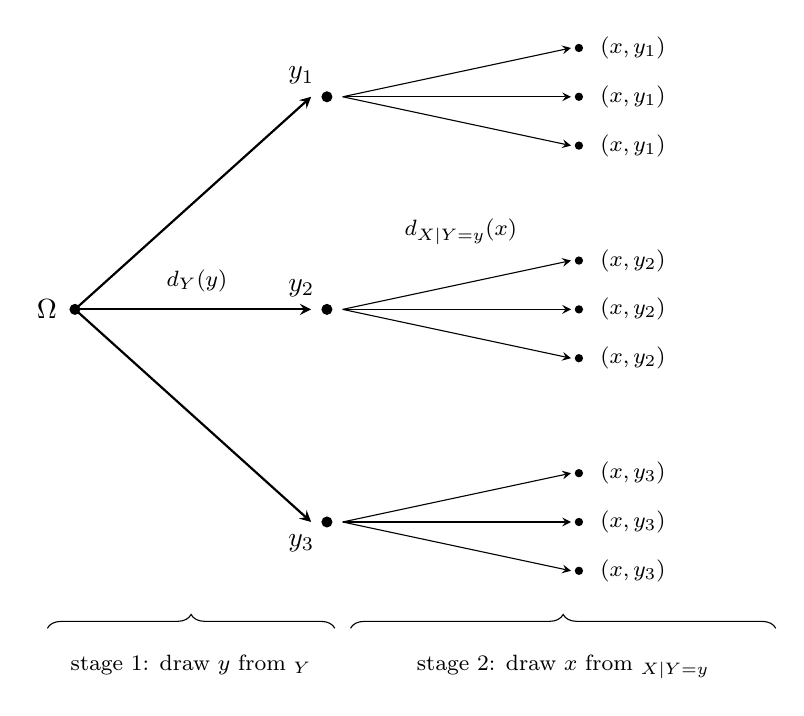
\begin{tikzpicture}[>=stealth, scale=1.0]
    % stage one
    \fill (0,0) circle (2pt) node[left=3pt] {$\Omega$};
    \draw[->, thick] (0,0) -- (3.0,2.7);
    \draw[->, thick] (0,0) -- (3.0,0.0);
    \draw[->, thick] (0,0) -- (3.0,-2.7);
    \node[above] at (1.55,0.1) {\footnotesize $d\prob_{Y}(y)$};
    \fill (3.2,2.7) circle (2pt) node[above left=1pt] {$y_{1}$};
    \fill (3.2,0.0) circle (2pt) node[above left=1pt] {$y_{2}$};
    \fill (3.2,-2.7) circle (2pt) node[below left=1pt] {$y_{3}$};
    % stage two
    \foreach \yy in {2.7,0.0,-2.7} {
      \draw[->] (3.4,\yy) -- (6.3,\yy+0.62);
      \draw[->] (3.4,\yy) -- (6.3,\yy);
      \draw[->] (3.4,\yy) -- (6.3,\yy-0.62);
      \fill (6.4,\yy+0.62) circle (1.5pt);
      \fill (6.4,\yy) circle (1.5pt);
      \fill (6.4,\yy-0.62) circle (1.5pt);
    }
    \foreach \yy/\lab in {2.7/1, 0.0/2, -2.7/3} {
      \node[right] at (6.55,\yy+0.62) {\footnotesize $(x,y_{\lab})$};
      \node[right] at (6.55,\yy) {\footnotesize $(x,y_{\lab})$};
      \node[right] at (6.55,\yy-0.62) {\footnotesize $(x,y_{\lab})$};
    }
    \node[above] at (4.9,0.7) {\footnotesize $d\prob_{X \mid Y = y}(x)$};
    % braces
    \draw[decorate, decoration={brace, amplitude=5pt}] (-0.35,-4.05) -- (3.3,-4.05)
      node[midway, below=6pt] {\footnotesize stage 1: draw $y$ from $\prob_{Y}$};
    \draw[decorate, decoration={brace, amplitude=5pt}] (3.5,-4.05) -- (8.9,-4.05)
      node[midway, below=6pt] {\footnotesize stage 2: draw $x$ from $\prob_{X \mid Y = y}$};
  \end{tikzpicture}
\end{figure}

The tree is the picture of the proposition. A point is produced in two stages,
and the probability of a set $C$ is obtained by integrating, over the first
stage, the probabilité conditionnelle computed at the second --- which with
$\phi = \indic_{C}$ is the displayed identity, and with a general $\phi$ is
the tower property of the last subsection.

\begin{prop}[Indépendance]
  Les variables aléatoires $X$ et $Y$ sont indépendantes si et seulement si la loi
  conditionnelle de $X$ sachant $Y = y$ est la loi de $X$ pour $\prob_{Y}$-presque
  tout $y$.
\end{prop}

Les variables aléatoires $X$ et $Y$ sont indépendantes si et seulement si
$\prob_{X,Y}(A \times B) = \prob_{X}(A) \prob_{Y}(B)$ for every borélien $A$ and every
$B \in \mathcal{E}$, ce qui est équivalent --- by the definition of the loi
conditionnelle --- à :
\[
  \forall A \in \mathcal{B}(\reals), \;\; \forall B \in \mathcal{E}, \qquad
  \int_{B} \prob_{X \mid Y = y}(A) \, d\prob_{Y}(y) \;=\; \int_{B} \prob_{X}(A) \, d\prob_{Y}(y) ,
\]
and p.p.\ uniqueness of densités turns the equality of the integrals into
$\prob_{X \mid Y = y}(A) = \prob_{X}(A)$ for $\prob_{Y}$-almost every $y$. So
indépendance is exactly the statement that conditioning on $Y$ teaches nothing
about $X$.

\begin{prop}[Condition sur une variable qui détermine l'autre]
  Si $X = \phi(Y)$ pour une certaine fonction mesurable $\phi$, alors la loi
  conditionnelle de $X$ sachant $Y = y$ est la mesure de Dirac en $\phi(y)$ pour
  $\prob_{Y}$-presque tout $y$.
\end{prop}

Indeed, for every borélien $A$ and every $B \in \mathcal{E}$,
\[
  \prob_{X,Y}(A \times B) \;=\; \prob(\phi(Y) \in A, \, Y \in B)
  \;=\; \int_{B} \indic_{A}(\phi(y)) \, d\prob_{Y}(y) ,
\]
on en déduit que pour $\prob_{Y}$-presque tout $y$,
$\prob_{X \mid Y = y}(A) = \indic_{A}(\phi(y)) = \delta_{\phi(y)}(A)$. The two
propositions are the two extremes of the same scale: knowing $Y$ tells nothing
about $X$ (indépendance, the loi conditionnelle is the unconditional one), or
knowing $Y$ tells everything (the loi conditionnelle is a point mass).

\begin{example}[The square of a uniform variable, given the variable]
  Soit $X$ une variable aléatoire de loi uniforme sur $[0,1]$. Pour presque tout
  $x \in [0,1]$, la loi conditionnelle de $X^{2}$ sachant $X = x$ est une mesure de
  Dirac en $x^{2}$. There is no randomness left to describe once $X$ is known, and
  the loi conditionnelle records that by collapsing to a point.
\end{example}

\subsection{Cas des lois à densité}

The general construction is not a recipe. It becomes one as soon as the loi jointe
has a densité, and that is the situation of every computation in this course.
On considère maintenant le cas de variables aléatoires réelles $X$, $Y$ dont la loi
jointe a une densité $f_{X,Y}$ par rapport à la mesure de Lebesgue de $\reals^{2}$.
Les variables aléatoires $X$ et $Y$ ont donc des densités par rapport à la mesure de
Lebesgue sur $\reals$, each obtained as usual by integrating out the other variable.

\begin{definition}[Densité conditionnelle]
  Pour tout réel $y$ tel que $f_{Y}(y) > 0$, on définit la \textbf{densité
  conditionnelle} (\textit{conditional density}) de la variable aléatoire $X$ par
  rapport à $Y = y$ comme la fonction $f_{X \mid Y = y}$ définie par :
  \[
    \forall x \in \reals, \qquad
    f_{X \mid Y = y}(x) \;=\; \frac{f_{X,Y}(x,y)}{f_{Y}(y)} .
  \]
\end{definition}

The condition $f_{Y}(y) > 0$ is part of the definition and not a side remark: at a
$y$ where the marginal densité vanishes the quotient is $0/0$ and no densité
conditionnelle is defined there. This is the trace, at the level of densités, of the
``$\prob_{Y}$-presque tout $y$'' of the previous subsection, since
$\{f_{Y} = 0\}$ carries no $\prob_{Y}$-mass. On vérifie que la loi conditionnelle a
bien pour densité cette fonction par rapport à la mesure de Lebesgue --- a short
verification. For all $A, B \in \mathcal{B}(\reals)$,
\begin{align*}
  \prob_{X,Y}(A \times B)
  &= \int_{A \times B} f_{X,Y}(x,y) \, dx \, dy \\
  &= \int_{A \times B} f_{X \mid Y = y}(x) f_{Y}(y) \, dx \, dy \\
  &= \int_{B} \left( \int_{A} f_{X \mid Y = y}(x) \, dx \right) f_{Y}(y) \, dy ,
\end{align*}
where the middle line is legitimate because on $\{f_{Y} = 0\}$ one has
$\int f_{X,Y}(x,y) \, dx = f_{Y}(y) = 0$, so that set of $y$ contributes nothing
to either side of the identity, and the last line is Tonelli, applicable
because the integrand is positive. Comparing with the defining identity of the
loi conditionnelle gives, pour $\prob_{Y}$-presque tout $y$,
\[
  \forall A \in \mathcal{B}(\reals), \qquad
  \prob_{X \mid Y = y}(A) \;=\; \int_{A} f_{X \mid Y = y}(x) \, dx .
\]

\begin{remark}
  Two extensions come free and both are used constantly. Les résultats s'étendent
  sans difficulté au cas où la loi jointe a une densité par rapport à une mesure
  \emph{produit} quelconque, not only Lebesgue$\,\otimes\,$Lebesgue (par exemple, le
  produit de la mesure de Lebesgue sur $\reals$ et d'une mesure discrète --- the
  important case being the mesure de comptage
  $\mu = \sum_{n \in \mathbb{N}} \delta_{n}$ on $\mathbb{N}$, which is what one
  needs when one variable is discrete and the other continuous), ainsi qu'au cas où
  $X$ et $Y$ sont des vecteurs aléatoires. The formula
  $f_{X \mid Y = y} = f_{X,Y}/f_{Y}$ is unchanged in both cases; only the reference
  mesure changes, and with it the meaning of ``densité''.
\end{remark}

\begin{remark}
  A practical consequence: at fixed $y$, $f_{X \mid Y = y}$ is proportional to
  $f_{X,Y}(\cdot,y)$, the constant being whatever makes it integrate to $1$. So
  one writes $f_{X \mid Y = y}(x) \propto f_{X,Y}(x,y)$, recognises the shape of a
  standard loi in $x$, and reads its normalisation off a table rather than
  computing $f_{Y}$. Most solutions below are obtained this way.
\end{remark}

\begin{example}[The smaller of two uniform draws, given the larger]
  Return to $X = \min(U,V)$ and $Y = \max(U,V)$ with $U,V$ independent uniform on
  $[0,1]$. Pour toute fonction mesurable positive $\phi$ --- a fonction test ---
  \[
    \expec(\phi(X,Y)) = \int \phi(\min(u,v),\max(u,v)) \indic_{]0,1[}(u) \indic_{]0,1[}(v) \, du \, dv
    = 2 \int \phi(x,y) \indic_{\Delta}(x,y) \, dx \, dy
  \]
  avec $\Delta = \{(x,y) \in [0,1]^{2} : x \leq y\}$, the factor $2$ coming from
  the two orderings of the pair. So la loi jointe a pour densité :
  \[
    f_{X,Y}(x,y) \;=\; 2 \times \indic_{\Delta}(x,y) ,
  \]
  la loi de $Y$ a pour densité $f_{Y}(y) = 2y \indic_{[0,1]}(y)$, and for every
  $y \in \;]0,1]$
  \[
    f_{X \mid Y = y}(x) \;=\; \frac{\indic_{\Delta}(x,y)}{y} ,
  \]
  c'est une loi uniforme sur $[0,y]$. The guess made when the example was
  introduced is confirmed, and $y = 0$ --- the single point where $f_{Y}$ vanishes
  --- is excluded, as the definition requires.
\end{example}

\begin{figure}[h!]
  \centering
  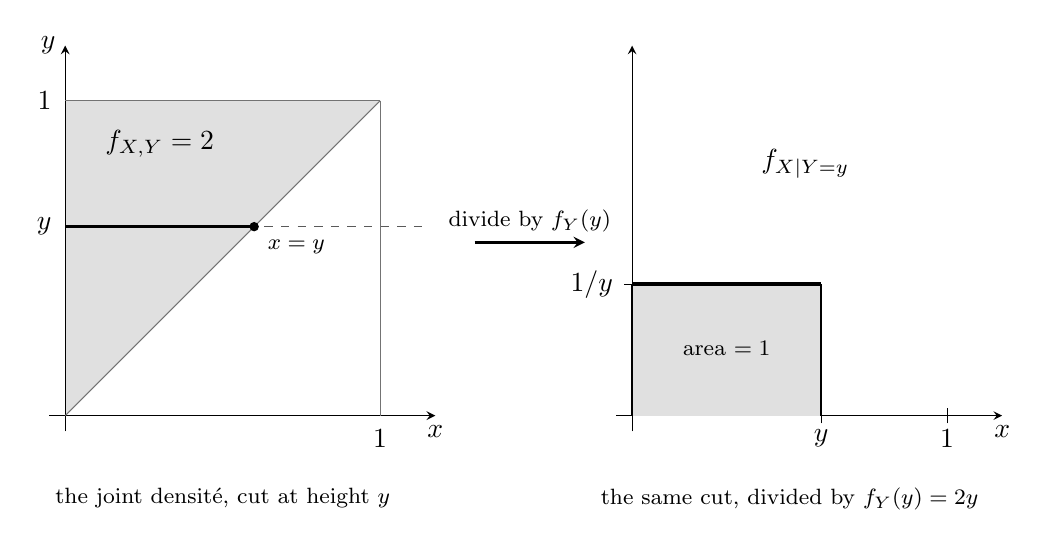
\begin{tikzpicture}[>=stealth, scale=1.0]
    % ---- left panel: the joint density on the triangle, sliced
    \fill[black!12] (0,0) -- (0,4) -- (4,4) -- cycle;
    \draw[->] (-0.2,0) -- (4.7,0) node[below] {$x$};
    \draw[->] (0,-0.2) -- (0,4.7) node[left] {$y$};
    \draw[thin,black!55] (0,0) -- (4,4);
    \draw[thin,black!55] (0,4) -- (4,4);
    \draw[thin,black!55] (4,0) -- (4,4);
    \node at (1.2,3.45) {$f_{X,Y} = 2$};
    \node[below] at (4,-0.05) {$1$};
    \node[left] at (-0.05,4) {$1$};
    % the slice
    \draw[dashed,black!65] (0,2.4) -- (4.6,2.4);
    \draw[very thick] (0,2.4) -- (2.4,2.4);
    \fill (2.4,2.4) circle (1.7pt);
    \node[left] at (-0.05,2.4) {$y$};
    \node[below right] at (2.45,2.35) {\footnotesize $x = y$};
    \node[below] at (2.0,-0.8) {\footnotesize the joint densité, cut at height $y$};
    % ---- right panel: the renormalised slice
    \begin{scope}[xshift=7.2cm]
      \draw[->] (-0.2,0) -- (4.7,0) node[below] {$x$};
      \draw[->] (0,-0.2) -- (0,4.7) node[left] {};
      \fill[black!12] (0,0) rectangle (2.4,1.67);
      \draw[very thick] (0,1.67) -- (2.4,1.67);
      \draw[thick] (0,0) -- (0,1.67);
      \draw[thick] (2.4,0) -- (2.4,1.67);
      \draw (-0.1,1.67) -- (0.1,1.67);
      \node[left] at (-0.12,1.67) {$1/y$};
      \draw (2.4,-0.1) -- (2.4,0.1);
      \node[below] at (2.4,-0.05) {$y$};
      \draw (4,-0.1) -- (4,0.1);
      \node[below] at (4.0,-0.05) {$1$};
      \node at (1.2,0.85) {\footnotesize area $= 1$};
      \node at (2.2,3.2) {$f_{X \mid Y = y}$};
      \node[below] at (2.0,-0.8) {\footnotesize the same cut, divided by $f_{Y}(y) = 2y$};
    \end{scope}
    % the arrow between panels
    \draw[->, thick] (5.2,2.2) -- (6.6,2.2)
      node[midway,above] {\footnotesize divide by $f_{Y}(y)$};
  \end{tikzpicture}
\end{figure}

The figure is the whole of this subsection in one image. Conditioning on
$Y = y$ means cutting the joint densité along the horizontal line at height $y$
and reading the profile of the cut as a function of $x$; that profile is
$f_{X,Y}(\cdot,y)$, not a probability densité, since it integrates to $f_{Y}(y)$
rather than $1$. Dividing by $f_{Y}(y)$ renormalises it. The picture also makes
the restriction $f_{Y}(y) > 0$ visible: where the cut meets the support in a set
of mesure zero there is nothing to renormalise.

\begin{prop}[Indépendance pour un couple à densité]
  Deux variables aléatoires $X, Y$ dont la loi jointe a une densité sont
  indépendantes si et seulement si la densité conditionnelle $f_{X \mid Y = y}$ est
  égale à la densité $f_{X}$, pour tout $y$ tel que $f_{Y}(y) > 0$.
\end{prop}

By the chapter 4 criterion, a pair with a joint densité is independent if and
only if $f_{X,Y}(x,y) = f_{X}(x) f_{Y}(y)$ p.p., which is to say
\[
  f_{X \mid Y = y}(x) f_{Y}(y) \;=\; f_{X}(x) f_{Y}(y)
\]
for Lebesgue-almost every $x$, at almost every $y$ with $f_{Y}(y) > 0$. Dividing by
$f_{Y}(y)$, which is legitimate exactly on that set of $y$, gives the claim.
A densité is only defined up to a set of mesure zero, so ``pour tout $y$'' is
to be read for a suitable choice of the densities; for an arbitrary choice the
equality holds p.p.\ in $y$ on the set where $f_{Y}(y) > 0$.

\begin{example}[A point drawn uniformly in the unit disc]
  Soit $A$ un point choisi de manière aléatoire et uniforme dans le disque unité
  $D$, centred at the origin. On note $(X,Y)$ ses coordonnées cartésiennes. La
  densité du vecteur est donnée par $f_{X,Y} = \tfrac{1}{\pi} \indic_{D}$, so for
  $x \in \;]-1,1[$,
  \[
    f_{Y \mid X = x}(y) \;\propto\; \indic_{D}(x,y)
    \;=\; \indic_{]-\sqrt{1-x^{2}}, \sqrt{1-x^{2}}[}(y) ,
  \]
  c'est une loi uniforme sur $]-\sqrt{1-x^{2}}, \sqrt{1-x^{2}}[$. The coordinates
  are not independent: the loi conditionnelle depends on $x$, and the proposition
  above says that is already enough to rule indépendance out. Espérance
  conditionnelle of a non-linear function is read off the same loi: by symmetry
  \[
    \expec(Y^{2} \mid X = x)
    \;=\; \int_{0}^{\sqrt{1-x^{2}}} y^{2} \, \frac{dy}{\sqrt{1-x^{2}}}
    \;=\; \frac{1-x^{2}}{3} ,
  \]
  so the disc centred at the origin and passing through $A$ has mean area
  \[
    \expec\big( \pi (X^{2} + Y^{2}) \,\big|\, X = x \big)
    \;=\; \pi x^{2} + \pi \, \frac{1-x^{2}}{3}
    \;=\; \frac{\pi}{3} (1 + 2x^{2}) .
  \]
\end{example}

\begin{example}[A uniform variable given its product with another]
  Soit $U$ et $V$ deux variables aléatoires i.i.d.\ de loi uniforme sur $]0,1[$, and
  set $T = UV$. Pour toute fonction mesurable positive $\phi$, the changement de
  variable $t = uv$ at fixed $u$ gives
  \[
    \expec(\phi(U,T)) = \int \phi(u,uv) \indic_{]0,1[}(u) \indic_{]0,1[}(v) \, du \, dv
    = \int \phi(u,t) \indic_{\Delta}(u,t) \, \frac{du}{u} \, dt
  \]
  avec $\Delta = \{(u,t) : 0 < t < u < 1\}$. On en déduit la densité
  $f_{U,T}(u,t) = \indic_{\Delta}(u,t)/u$.
  Hence, for $t \in \;]0,1[$,
  \[
    f_{U \mid T = t}(u) \;\propto\; \frac{\indic_{]t,1[}(u)}{u} ,
    \qquad \int \frac{\indic_{]t,1[}(u)}{u} \, du = -\ln t ,
    \qquad\text{so}\qquad
    f_{U \mid T = t}(u) \;=\; -\frac{\indic_{]t,1[}(u)}{u \ln t} .
  \]
  The loi conditionnelle is not uniform, which is worth seeing once: conditioning on
  a smooth function of the pair does not in general leave a loi from the
  standard tables. Integrating gives
  $\expec(U \mid UV = \tfrac{1}{2}) = 1/(2\ln 2)$.
\end{example}

\subsection{Espérance conditionnelle}

On étend la définition de l'espérance conditionnelle à une condition sur une
variable aléatoire, in place of the condition on an événement of the first
subsection. Cette généralisation n'est pas immédiate car la loi conditionnelle
$\prob_{X \mid Y = y}$ est une mesure de probabilité sur $(\reals,\mathcal{B}(\reals))$
et non sur l'espace de probabilité $(\Omega,\mathcal{F})$, où sont définies les
variables aléatoires $X$ et $Y$ --- a mismatch of spaces --- so
$\int X \, d\prob_{X \mid Y = y}$ is not a well-formed expression and the first
definition cannot simply be copied. On peut par contre calculer l'espérance de toute
fonction mesurable de $X$ et $Y$: integrate it against the loi conditionnelle, in
the variable $x$, at a fixed $y$.

\begin{definition}[Espérance conditionnelle sachant $Y = y$]
  Pour $\prob_{Y}$-presque tout $y$, on définit l'espérance conditionnelle de
  $\phi(X,Y)$ sachant $Y = y$ comme :
  \[
    \expec(\phi(X,Y) \mid Y = y) \;=\; \int \phi(x,y) \, d\prob_{X \mid Y = y}(x) ,
  \]
  dès que cette intégrale est bien définie.
\end{definition}

Two qualifications travel with this definition and neither is decorative. The
$\prob_{Y}$-presque tout $y$ is inherited from the loi conditionnelle, which is
itself only defined $\prob_{Y}$-presque partout. And ``dès que cette intégrale
est bien définie'' is the chapter 3 caveat again: the integral must not be an
$\infty - \infty$.\\

The bridge back to the first subsection closes here. On retrouve bien l'espérance
conditionnelle lorsque la condition porte sur un événement $A \in \mathcal{F}$ de
probabilité non nulle, $\prob(A) > 0$. Avec $Y = \indic_{A}$ --- and
$\phi(x,y) = x$ --- on obtient en effet :
\[
  \expec(X \mid A) \;=\; \expec(X \mid Y = 1) \;=\; \int x \, d\prob_{X \mid A}(x) ,
\]
which is exactly the form the théorème de transfert gives to the espérance
conditionnelle given an événement. So the general definition restricts correctly,
and the discrete espérance conditionnelle of chapter 1 is a special case of a
special case.

\begin{theorem}[Calcul d'espérance par conditionnement]
  On a :
  \[
    \expec(\phi(X,Y)) \;=\; \int \expec(\phi(X,Y) \mid Y = y) \, d\prob_{Y}(y) ,
  \]
  pour toute fonction mesurable $\phi$ positive ou telle que
  $\expec(|\phi(X,Y)|) < \infty$.
\end{theorem}

\begin{proof}
  The argument is the standard four-rung ladder of this course --- indicator,
  étagée, positive mesurable, general --- the same one that carried the théorème
  de transfert and the integration of a mesure à densité in chapter 3. Only the
  bottom rung contains anything specific to conditioning.\\

  \textbf{Fonctions indicatrices.} Soit $\phi = \indic_{C}$ avec
  $C \in \mathcal{B}(\reals) \otimes \mathcal{E}$. By the proposition on the loi
  jointe,
  \begin{align*}
    \expec(\phi(X,Y)) &= \prob_{X,Y}(C) \\
    &= \int \left( \int \indic_{C}(x,y) \, d\prob_{X \mid Y = y}(x) \right) d\prob_{Y}(y) \\
    &= \int \expec(\phi(X,Y) \mid Y = y) \, d\prob_{Y}(y) ,
  \end{align*}
  the last line being the definition of the espérance conditionnelle read
  backwards.\\

  \textbf{Fonctions étagées positives.} A fonction étagée positive is a finite
  positive combination $\phi = \sum_{k} a_{k} \indic_{C_{k}}$, and both sides
  of the identity are linear in $\phi$ --- the left by linearity of the
  espérance, the right by linearity of both integrals --- so le résultat s'étend à
  toute fonction étagée positive par linéarité.\\

  \textbf{Fonctions mesurables positives.} Any positive mesurable $\phi$ is
  the increasing limit of a sequence of fonctions étagées positives, and le
  résultat s'étend à toute fonction mesurable positive par convergence monotone: it
  applies on the left, and twice on the right --- once in $x$ for each fixed $y$,
  once in $y$ --- so the identity passes to the limit.\\

  \textbf{Le cas général.} For $\phi$ with $\expec(|\phi(X,Y)|) < \infty$,
  on applique le résultat aux fonctions $\phi^{+}$ et $\phi^{-}$, separately, and
  subtract. The integrability hypothesis is what makes the subtraction legitimate:
  both terms are finite, so no $\infty - \infty$ arises.
\end{proof}

\begin{remark}
  The hypothesis ``positive ou telle que $\expec(|\phi(X,Y)|) < \infty$'' is the
  same dichotomy that runs through every convergence and exchange statement of
  chapter 3, and it is not weakenable. Drop it and the two sides can both fail to
  be defined. Note also that the integrability is asked of
  $\phi(X,Y)$ --- a statement about the loi jointe --- and not of the espérance
  conditionnelle.
\end{remark}

\begin{remark}
  The function $y \mapsto \expec(\phi(X,Y) \mid Y = y)$ can be shown to be
  mesurable. This course states the fact and does not prove it; the proof is of a
  piece with the théorème de Jirina, since a mesurable choice of the loi
  conditionnelle is what makes a mesurable espérance conditionnelle available.
  Everything below rests on it: without it, substituting $Y(\omega)$ for $y$ would
  not produce a variable aléatoire and the concise form of the theorem could not be
  written.
\end{remark}

Comme l'espérance conditionnelle $\expec(\phi(X,Y) \mid Y = y)$ est une fonction de
$y$, dont on peut montrer qu'elle est mesurable --- the fact just granted --- on peut
en faire une variable aléatoire, notée $\expec(\phi(X,Y) \mid Y)$, en remplaçant
$y$ par $Y(\omega)$, une fonction de $\omega \in \Omega$. Le théorème précédent
s'écrit alors de manière concise comme suit :
\[
  \expec(\phi(X,Y)) \;=\; \expec\big( \expec(\phi(X,Y) \mid Y) \big) ,
\]
and in particular, taking $\phi(x,y) = x$,
\begin{equation*}
  \boxed{\;\expec(X) \;=\; \expec\big( \expec(X \mid Y) \big)\;}
\end{equation*}
dès que la variable aléatoire $X$ est positive ou intégrable. This is the
\textbf{tower property}, and it is the single most used identity of the chapter:
it computes an espérance by first
conditioning on whatever makes the problem easy, then averaging the answer.

\begin{remark}
  Notice the type discipline. $\expec(X \mid A)$ is a number;
  $\expec(X \mid Y = y)$ is a number for each fixed $y$;
  $\expec(X \mid Y)$ is a \emph{variable aléatoire}, the composition of the function
  $y \mapsto \expec(X \mid Y = y)$ with $Y$. Only the third can be put inside an
  outer espérance, and mixing the three is the most common way of writing a
  false line in this chapter.
\end{remark}

\begin{example}[Recovering the espérance of a minimum by conditioning]
  With $X = \min(U,V)$ and $Y = \max(U,V)$ as before, la loi de $X$ sachant $Y = y$
  étant uniforme sur $[0,y]$, on a $\expec(X \mid Y = y) = y/2$, d'où
  $\expec(X \mid Y) = Y/2$ as a variable aléatoire. Since
  $f_{Y}(y) = 2y \indic_{[0,1]}(y)$ gives $\expec(Y) = 2/3$, the tower property
  yields
  \[
    \expec(X) \;=\; \expec\big( \expec(X \mid Y) \big) \;=\; \expec\!\left( \frac{Y}{2} \right) \;=\; \frac{1}{3} ,
  \]
  which is indeed the espérance of the minimum, since
  $f_{X}(x) = 2(1-x)\indic_{]0,1[}(x)$. The same loi conditionnelle answers questions
  that are not espérances: for instance
  $\prob(X + Y \leq 1 \mid Y = \tfrac{3}{4}) = \prob(X \leq \tfrac{1}{4} \mid Y = \tfrac{3}{4}) = \tfrac{1}{3}$,
  by measuring $[0,\tfrac{1}{4}]$ under the loi uniforme on $[0,\tfrac{3}{4}]$.
\end{example}

\begin{remark}
  Le théorème généralise l'équivalent de la formule des probabilités totales pour
  l'espérance, seen in the first subsection, which it contains as a special case.
  Soit $(A_{i})_{i \in I}$ une famille d'événements formant une partition de
  $\Omega$, avec $\prob(A_{i}) > 0$ pour tout $i$ et $I \subr \mathbb{N}$. En
  définissant $Y = \sum_{i \in I} i \, \indic_{A_{i}}$, the variable aléatoire that
  reports which block of the partition occurred, so that $\{Y = i\} = A_{i}$, on
  obtient :
  \[
    \expec(X) \;=\; \expec\big( \expec(X \mid Y) \big)
    \;=\; \sum_{i \in I} \prob(Y = i) \expec(X \mid Y = i)
    \;=\; \sum_{i \in I} \prob(A_{i}) \expec(X \mid A_{i}) ,
  \]
  the middle equality because the loi of $Y$ is the discrete mesure
  $\sum_{i} \prob(A_{i}) \delta_{i}$, so an integral against $\prob_{Y}$ is a sum.
\end{remark}

Dans le cas où la loi jointe de $X$ et $Y$ a une densité par rapport à la mesure de
Lebesgue, le théorème s'écrit, in the form one actually computes with :
\begin{equation*}
  \expec(\phi(X,Y)) \;=\; \int \left( \int \phi(x,y) f_{X \mid Y = y}(x) \, dx \right) f_{Y}(y) \, dy
\end{equation*}
pour toute fonction mesurable $\phi$ positive ou telle que
$\expec(|\phi(X,Y)|) < \infty$. The inner integral is
$\expec(\phi(X,Y) \mid Y = y)$; the outer one averages it over $y$. As with the
densité conditionnelle itself, the formula survives the replacement of the mesure
de Lebesgue by any mesure produit, with sums replacing integrals in the discrete
directions.

\begin{example}[A power of a uniform variable with a Bernoulli exponent]
  Soit $X \sim \mathcal{B}(p)$, une variable aléatoire suivant une loi de Bernoulli
  de paramètre $p \in \;]0,1[$, et $Y$ une variable aléatoire suivant une loi
  uniforme sur $[0,1]$, indépendante de $X$. Conditioning on $X$ --- a variable
  with two atoms, so the elementary case --- gives
  \[
    \expec(Y^{X} \mid X = 0) = \expec(1) = 1 ,
    \qquad
    \expec(Y^{X} \mid X = 1) = \expec(Y) = \frac{1}{2} ,
  \]
  where the indépendance of $X$ and $Y$ is what allows $\prob_{Y \mid X = x}$ to be
  replaced by $\prob_{Y}$. The tower property then gives
  \[
    \expec(Y^{X}) \;=\; (1-p) \cdot 1 + p \cdot \frac{1}{2} \;=\; 1 - \frac{p}{2} ,
  \]
  and as a variable aléatoire
  $\expec(Y^{X} \mid X) = 1 - X + \tfrac{X}{2} = 1 - \tfrac{X}{2}$, a function of
  $X$ as the type discipline demands.
\end{example}

\begin{example}[Conditioning inside a triangle]
  Soit $(X,Y)$ le vecteur aléatoire réel de densité $f_{X,Y} = 2 \times \indic_{\Delta}$
  avec $\Delta = \{(x,y) \in \reals_{+}^{2} : x + y \leq 1\}$. For $x \in \;]0,1[$,
  \[
    f_{Y \mid X = x}(y) \;\propto\; \indic_{\Delta}(x,y) \;\propto\; \indic_{]0,1-x[}(y) ,
    \qquad\text{so}\qquad
    f_{Y \mid X = x}(y) \;=\; \frac{\indic_{]0,1-x[}(y)}{1-x} ,
  \]
  c'est une loi uniforme sur $]0,1-x[$, whence $\expec(Y \mid X = x) = (1-x)/2$. The
  normalising constant was read off from the shape of the indicator without ever
  computing $f_{X}$, which is the working method of the previous remark.
\end{example}

\begin{example}[A win rate inferred from a run of games]
  La fréquence de gain à un jeu, notée $X$, est supposée être une variable aléatoire
  de loi uniforme sur $[0,1]$. Soit $N$ le nombre de parties gagnées sur $n$
  tentatives: la loi de $N$ sachant $X = x$ suit une loi binomiale
  $\mathcal{B}(n,x)$, soit :
  \[
    \prob(N = k \mid X = x) \;=\; \binom{n}{k} x^{k} (1-x)^{n-k} .
  \]
  C'est la densité conditionnelle de $N$ sachant $X = x$ par rapport à la mesure de
  comptage $\mu = \sum_{k \in \mathbb{N}} \delta_{k}$. Le couple $(X,N)$ a donc pour
  densité :
  \[
    f_{X,N}(x,k) \;=\; \indic_{[0,1]}(x) \binom{n}{k} x^{k} (1-x)^{n-k}
  \]
  par rapport à la mesure produit $\lambda \otimes \mu$. Reading the quotient
  in the other direction,
  \[
    f_{X \mid N = k}(x) \;\propto\; \indic_{[0,1]}(x) \, x^{k} (1-x)^{n-k} ,
  \]
  on reconnaît une loi Beta $\mathcal{B}(k+1, n-k+1)$. Conditioning has
  been reversed: the model was specified as ``$X$, then $N$ given $X$'', and what
  is wanted is ``$X$ given $N$''. The joint densité, which does not care which
  variable came first, is the object that permits the reversal.
\end{example}

\begin{example}[A geometric count paired with an exponential time]
  Fix $a > 0$ and $b > 0$ and let $(X,Y)$ take values in
  $\mathbb{N} \times \reals_{+}$ with loi characterised by
  \[
    \forall n \in \mathbb{N}, \; \forall t \in \reals_{+}, \qquad
    \prob(X = n, \, Y \leq t) \;=\; b \int_{0}^{t} \frac{(ay)^{n}}{n!} e^{-(a+b)y} \, dy .
  \]
  The pair has densité
  $f_{X,Y}(n,t) = b \frac{(at)^{n}}{n!} e^{-(a+b)t} \indic_{\reals_{+}}(t)$
  with respect to $\mu \otimes \lambda$, where
  $\mu = \sum_{n \in \mathbb{N}} \delta_{n}$ is the mesure de comptage on
  $\mathbb{N}$ and $\lambda$ is the mesure de Lebesgue. Integrating out $t$ gives
  the marginal of $X$,
  \[
    \prob(X = n) \;=\; \frac{b}{a+b} \left( \frac{a}{a+b} \right)^{n} ,
  \]
  a loi géométrique on $\mathbb{N}$ of parameter $b/(a+b)$, and summing over $n$
  gives $f_{Y}(t) = b e^{-bt} \indic_{\reals_{+}}(t)$, a loi $\mathcal{E}(b)$.
  Both conditionings are now quotients. In one direction,
  \[
    f_{Y \mid X = n}(t) \;=\; \frac{(a+b)^{n+1}}{n!} \, t^{n} e^{-(a+b)t} \indic_{\reals_{+}}(t) ,
  \]
  a loi Gamma $\Gamma(n+1, a+b)$, so that
  \[
    \expec(Y \mid X = n) \;=\; \frac{n+1}{a+b} ,
    \qquad
    \expec\!\left( \frac{Y}{X+1} \,\Big|\, X = n \right) \;=\; \frac{1}{n+1} \expec(Y \mid X = n) \;=\; \frac{1}{a+b} ,
  \]
  the factor $1/(n+1)$ coming out of the integral because it is constant once $X$
  is fixed at $n$, the variable of integration being the value of $Y$. The
  espérance conditionnelle being the same constant for every $n$, the tower
  property gives $\expec(Y/(X+1)) = 1/(a+b)$ without any further
  integration. In the other direction,
  \[
    \prob(X = n \mid Y = t) \;=\; \frac{(at)^{n}}{n!} e^{-at} ,
  \]
  a loi de Poisson $\mathcal{P}(at)$, and therefore $\expec(X \mid Y = t) = at$.
\end{example}

\begin{example}[Splitting an exponential sum into a proportion and a total]
  Let $U \sim \mathcal{E}(\lambda)$ and $V \sim \mathcal{E}(\mu)$ be independent,
  and set $X = U + V$ and $Y = U/(U+V)$. The changement de
  variable $u = xy$, $v = x(1-y)$, a diffeomorphism of
  $]0,+\infty[ \, \times \, ]0,1[$ onto $]0,+\infty[^{2}$ with Jacobian
  determinant of absolute value $x$, gives
  \[
    f_{X,Y}(x,y) \;=\; \lambda \mu \, x \, e^{-\mu x} e^{-(\lambda - \mu) x y}
      \indic_{]0,+\infty[}(x) \indic_{]0,1[}(y) .
  \]
  When $\lambda = \mu$ the exponential in $y$ disappears, the densité factorises
  as $\lambda^{2} x e^{-\lambda x} \indic_{]0,+\infty[}(x) \cdot \indic_{]0,1[}(y)$,
  and the two variables are independent: $X$ follows $\Gamma(2,\lambda)$ and $Y$
  is uniform on $[0,1]$, so $f_{Y \mid X = x} = f_{Y}$ as the indépendance
  criterion predicts. When $\lambda \neq \mu$ the marginal of $X$ is
  \[
    f_{X}(x) \;=\; \lambda \mu \, \frac{e^{-\lambda x} - e^{-\mu x}}{\mu - \lambda} \indic_{]0,+\infty[}(x) ,
  \]
  and dividing,
  \[
    f_{Y \mid X = x}(y) \;=\; x (\mu - \lambda) \frac{e^{(\mu - \lambda) x y}}{e^{(\mu - \lambda) x} - 1} \indic_{]0,1[}(y) ,
    \qquad x > 0 ,
  \]
  which depends on $x$, so the variables are not independent. Integrating this
  densité conditionnelle over $]0,\tfrac{1}{2}[$ gives
  \[
    \prob\!\left( Y \leq \tfrac{1}{2} \,\Big|\, X = x \right)
    \;=\; \frac{e^{(\mu - \lambda) x / 2} - 1}{e^{(\mu - \lambda) x} - 1}
    \;\xrightarrow[x \to +\infty]{}\;
    \begin{cases}
      0 & \text{if } \lambda < \mu, \\
      1 & \text{if } \lambda > \mu,
    \end{cases}
  \]
  with the value $\tfrac{1}{2}$ for every $x$ in the case $\lambda = \mu$. The
  interpretation is clean: conditionally on a very large total $U + V$, the
  slower-decaying component --- the one with the smaller rate, hence the heavier
  tail --- is the one that must have been large, so the proportion $Y$
  concentrates at $0$ or at $1$ according to which rate is bigger.
\end{example}

\begin{conclusion}
  A loi conditionnelle given an événement non négligeable is a mesure image and
  behaves like any other loi. A loi conditionnelle given a variable aléatoire is a
  densité of $B \mapsto \prob_{X,Y}(A \times B)$ with respect to
  $\prob_{Y}$ --- the one the théorème de Radon-Nikodym provides --- defined for
  $\prob_{Y}$-almost every $y$, and existing simultaneously in $A$ only by the
  théorème de Jirina. When the loi jointe has a densité with respect to a mesure
  produit, the densité conditionnelle is the joint divided by the marginal wherever
  the marginal is strictly positive, and every computation reduces to reading a
  proportionality in $x$ at fixed $y$ and normalising. Espérance conditionnelle is an
  integral against the loi conditionnelle, and the tower property
  $\expec(X) = \expec(\expec(X \mid Y))$ turns conditioning into a method for
  computing espérances, valid for $X$ positive or integrable.
\end{conclusion}
